\documentclass[twoside]{book}

% Packages required by doxygen
\usepackage{fixltx2e}
\usepackage{calc}
\usepackage{doxygen}
\usepackage[export]{adjustbox} % also loads graphicx
\usepackage{graphicx}
\usepackage[utf8]{inputenc}
\usepackage{makeidx}
\usepackage{multicol}
\usepackage{multirow}
\PassOptionsToPackage{warn}{textcomp}
\usepackage{textcomp}
\usepackage[nointegrals]{wasysym}
\usepackage[table]{xcolor}

% Font selection
\usepackage[T1]{fontenc}
\usepackage[scaled=.90]{helvet}
\usepackage{courier}
\usepackage{amssymb}
\usepackage{sectsty}
\renewcommand{\familydefault}{\sfdefault}
\allsectionsfont{%
  \fontseries{bc}\selectfont%
  \color{darkgray}%
}
\renewcommand{\DoxyLabelFont}{%
  \fontseries{bc}\selectfont%
  \color{darkgray}%
}
\newcommand{\+}{\discretionary{\mbox{\scriptsize$\hookleftarrow$}}{}{}}

% Page & text layout
\usepackage{geometry}
\geometry{%
  a4paper,%
  top=2.5cm,%
  bottom=2.5cm,%
  left=2.5cm,%
  right=2.5cm%
}
\tolerance=750
\hfuzz=15pt
\hbadness=750
\setlength{\emergencystretch}{15pt}
\setlength{\parindent}{0cm}
\setlength{\parskip}{3ex plus 2ex minus 2ex}
\makeatletter
\renewcommand{\paragraph}{%
  \@startsection{paragraph}{4}{0ex}{-1.0ex}{1.0ex}{%
    \normalfont\normalsize\bfseries\SS@parafont%
  }%
}
\renewcommand{\subparagraph}{%
  \@startsection{subparagraph}{5}{0ex}{-1.0ex}{1.0ex}{%
    \normalfont\normalsize\bfseries\SS@subparafont%
  }%
}
\makeatother

% Headers & footers
\usepackage{fancyhdr}
\pagestyle{fancyplain}
\fancyhead[LE]{\fancyplain{}{\bfseries\thepage}}
\fancyhead[CE]{\fancyplain{}{}}
\fancyhead[RE]{\fancyplain{}{\bfseries\leftmark}}
\fancyhead[LO]{\fancyplain{}{\bfseries\rightmark}}
\fancyhead[CO]{\fancyplain{}{}}
\fancyhead[RO]{\fancyplain{}{\bfseries\thepage}}
\fancyfoot[LE]{\fancyplain{}{}}
\fancyfoot[CE]{\fancyplain{}{}}
\fancyfoot[RE]{\fancyplain{}{\bfseries\scriptsize Generated by Doxygen }}
\fancyfoot[LO]{\fancyplain{}{\bfseries\scriptsize Generated by Doxygen }}
\fancyfoot[CO]{\fancyplain{}{}}
\fancyfoot[RO]{\fancyplain{}{}}
\renewcommand{\footrulewidth}{0.4pt}
\renewcommand{\chaptermark}[1]{%
  \markboth{#1}{}%
}
\renewcommand{\sectionmark}[1]{%
  \markright{\thesection\ #1}%
}

% Indices & bibliography
\usepackage{natbib}
\usepackage[titles]{tocloft}
\setcounter{tocdepth}{3}
\setcounter{secnumdepth}{5}
\makeindex

% Hyperlinks (required, but should be loaded last)
\usepackage{ifpdf}
\ifpdf
  \usepackage[pdftex,pagebackref=true]{hyperref}
\else
  \usepackage[ps2pdf,pagebackref=true]{hyperref}
\fi
\hypersetup{%
  colorlinks=true,%
  linkcolor=blue,%
  citecolor=blue,%
  unicode%
}

% Custom commands
\newcommand{\clearemptydoublepage}{%
  \newpage{\pagestyle{empty}\cleardoublepage}%
}

\usepackage{caption}
\captionsetup{labelsep=space,justification=centering,font={bf},singlelinecheck=off,skip=4pt,position=top}

%===== C O N T E N T S =====

\begin{document}

% Titlepage & ToC
\hypersetup{pageanchor=false,
             bookmarksnumbered=true,
             pdfencoding=unicode
            }
\pagenumbering{roman}
\begin{titlepage}
\vspace*{7cm}
\begin{center}%
{\Large Robust Sparse Signal Recovery Based On Weighted Median Operator \mbox{[}Reproducible Research\mbox{]} }\\
\vspace*{1cm}
{\large Generated by Doxygen 1.8.11}\\
\end{center}
\end{titlepage}
\clearemptydoublepage
\tableofcontents
\clearemptydoublepage
\pagenumbering{arabic}
\hypersetup{pageanchor=true}

%--- Begin generated contents ---
\chapter{File Index}
\section{File List}
Here is a list of all files with brief descriptions\+:\begin{DoxyCompactList}
\item\contentsline{section}{headers/\hyperlink{functions_8h}{functions.\+h} \\*Function prototypes for implementing robust sparse signal recovery algorithms based on the weighted median operator }{\pageref{functions_8h}}{}
\item\contentsline{section}{simulations/\hyperlink{nmse__vs__snr__econtaminated_8c}{nmse\+\_\+vs\+\_\+snr\+\_\+econtaminated.\+c} \\*C routine that generates the data for building the Figure 2(b) }{\pageref{nmse__vs__snr__econtaminated_8c}}{}
\item\contentsline{section}{simulations/\hyperlink{nmse__vs__snr__gaussian_8c}{nmse\+\_\+vs\+\_\+snr\+\_\+gaussian.\+c} \\*C routine that generates the data for building the Figure 2(a) }{\pageref{nmse__vs__snr__gaussian_8c}}{}
\item\contentsline{section}{simulations/\hyperlink{rsnr__vs__snr__implevel_8c}{rsnr\+\_\+vs\+\_\+snr\+\_\+implevel.\+c} \\*C routine that generates the data for building the Figure 2(c) }{\pageref{rsnr__vs__snr__implevel_8c}}{}
\end{DoxyCompactList}

\chapter{File Documentation}
\hypertarget{functions_8h}{}\section{headers/functions.h File Reference}
\label{functions_8h}\index{headers/functions.\+h@{headers/functions.\+h}}


Function prototypes for implementing robust sparse signal recovery algorithms based on the weighted median operator.  


{\ttfamily \#include $<$stdlib.\+h$>$}\\*
{\ttfamily \#include $<$stdio.\+h$>$}\\*
Include dependency graph for functions.\+h\+:

\hypertarget{nmse__vs__snr__econtaminated_8c}{}\section{simulations/nmse\+\_\+vs\+\_\+snr\+\_\+econtaminated.c File Reference}
\label{nmse__vs__snr__econtaminated_8c}\index{simulations/nmse\+\_\+vs\+\_\+snr\+\_\+econtaminated.\+c@{simulations/nmse\+\_\+vs\+\_\+snr\+\_\+econtaminated.\+c}}
{\ttfamily \#include $<$stdlib.\+h$>$}\\*
{\ttfamily \#include $<$stdio.\+h$>$}\\*
{\ttfamily \#include $<$time.\+h$>$}\\*
{\ttfamily \#include $<$math.\+h$>$}\\*
{\ttfamily \#include \char`\"{}../headers/functions.\+h\char`\"{}}\\*
Include dependency graph for nmse\+\_\+vs\+\_\+snr\+\_\+econtaminated.\+c\+:
% FIG 0
\subsection*{Functions}
\begin{DoxyCompactItemize}
\item 
int \hyperlink{nmse__vs__snr__econtaminated_8c_ae66f6b31b5ad750f1fe042a706a4e3d4}{main} ()
\end{DoxyCompactItemize}


\subsection{Function Documentation}
\index{nmse\+\_\+vs\+\_\+snr\+\_\+econtaminated.\+c@{nmse\+\_\+vs\+\_\+snr\+\_\+econtaminated.\+c}!main@{main}}
\index{main@{main}!nmse\+\_\+vs\+\_\+snr\+\_\+econtaminated.\+c@{nmse\+\_\+vs\+\_\+snr\+\_\+econtaminated.\+c}}
\subsubsection[{\texorpdfstring{main()}{main()}}]{\setlength{\rightskip}{0pt plus 5cm}int main (
\begin{DoxyParamCaption}
{}
\end{DoxyParamCaption}
)}\hypertarget{nmse__vs__snr__econtaminated_8c_ae66f6b31b5ad750f1fe042a706a4e3d4}{}\label{nmse__vs__snr__econtaminated_8c_ae66f6b31b5ad750f1fe042a706a4e3d4}

\hypertarget{nmse__vs__snr__gaussian_8c}{}\section{simulations/nmse\+\_\+vs\+\_\+snr\+\_\+gaussian.c File Reference}
\label{nmse__vs__snr__gaussian_8c}\index{simulations/nmse\+\_\+vs\+\_\+snr\+\_\+gaussian.\+c@{simulations/nmse\+\_\+vs\+\_\+snr\+\_\+gaussian.\+c}}


C routine that generates the data for building the Figure 2(a).  


{\ttfamily \#include $<$time.\+h$>$}\\*
{\ttfamily \#include $<$math.\+h$>$}\\*
{\ttfamily \#include \char`\"{}../headers/functions.\+h\char`\"{}}\\*
Include dependency graph for nmse\+\_\+vs\+\_\+snr\+\_\+gaussian.\+c\+:\nopagebreak
\begin{figure}[H]
\begin{center}
\leavevmode
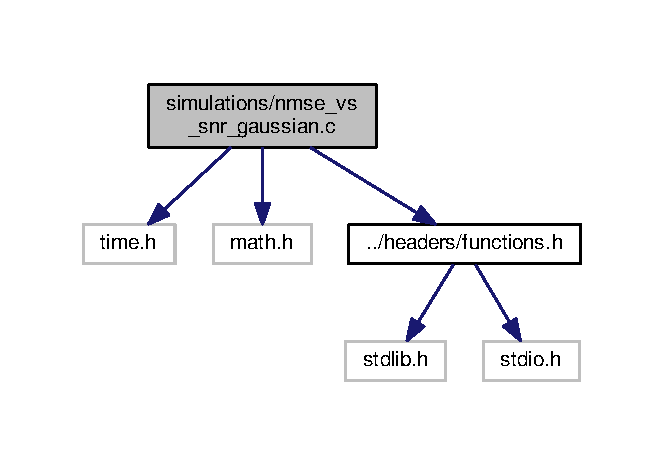
\includegraphics[width=319pt]{nmse__vs__snr__gaussian_8c__incl}
\end{center}
\end{figure}
\subsection*{Functions}
\begin{DoxyCompactItemize}
\item 
int \hyperlink{nmse__vs__snr__gaussian_8c_ae66f6b31b5ad750f1fe042a706a4e3d4}{main} ()
\end{DoxyCompactItemize}


\subsection{Detailed Description}
C routine that generates the data for building the Figure 2(a). 

Figure 2(a) shows the curves of the normalized mean square error (N\+M\+SE) in dB of the recovered coefficient vector versus the signal-\/to-\/noise ratio (S\+NR) in dB of the random projections. For this experiment, the additive perturbations are characterized as random samples that obeys to a zero mean Gaussian distribution. More precisely, the variance of the additive noise is computed from the S\+NR values under evaluation. Furthermore, this experiment obtains the error data generated by both the proposed sparse signal recovery algorithm (W\+M\+R-\/\+AR, weighted median regressions with adaptive regularizer) and the method based on weighted median regressions with hard thresholding (W\+M\+R-\/\+HT). Each point in the curves are obtained by averaging a user-\/defined number of trials, which is introduced in running time. The results of the simulation are saved in the results directory and the curves can be visualized by running the {\ttfamily Figure2a.\+m} routine. This plotting routine can be executed under either Octave or Matlab.

\begin{DoxyAuthor}{Author}
Juan Marcos Ramirez Rondon (\href{mailto:juanra@ula.ve}{\tt juanra@ula.\+ve}, \href{mailto:juanmarcos26@gmail.com}{\tt juanmarcos26@gmail.\+com}) 
\end{DoxyAuthor}
\begin{DoxyDate}{Date}
August, 2017 
\end{DoxyDate}
\begin{DoxyVersion}{Version}
1.\+00 
\end{DoxyVersion}
\begin{DoxySeeAlso}{See also}
Ramirez, J. M., \& Paredes, J. L. (2014). Robust Sparse Signal Recovery Based on Weighted Median Operator. I\+E\+EE International Conference on Acoustic, Speech, and Signal Processing (I\+C\+A\+S\+SP 2014). pp 1050-\/1054. Available on\+: \href{https://github.com/JuanMarcosRamirez/SparseRecoveryWeightedMedian/blob/master/p1050-ramirez.pdf}{\tt https\+://github.\+com/\+Juan\+Marcos\+Ramirez/\+Sparse\+Recovery\+Weighted\+Median/blob/master/p1050-\/ramirez.\+pdf} 

Paredes, J. L., \& Arce, G. R. (2011). Compressive sensing signal reconstruction by weighted median regression estimates. I\+E\+EE Transactions on Signal Processing, 59(6), 2585-\/2601. Available on\+: \href{https://www.eecis.udel.edu/~arce/Group/Entries/2012/7/2_Compressive_Spectral_Imaging_files/CompSignReconst.pdf}{\tt https\+://www.\+eecis.\+udel.\+edu/$\sim$arce/\+Group/\+Entries/2012/7/2\+\_\+\+Compressive\+\_\+\+Spectral\+\_\+\+Imaging\+\_\+files/\+Comp\+Sign\+Reconst.\+pdf}
\end{DoxySeeAlso}
 

\subsection{Function Documentation}
\index{nmse\+\_\+vs\+\_\+snr\+\_\+gaussian.\+c@{nmse\+\_\+vs\+\_\+snr\+\_\+gaussian.\+c}!main@{main}}
\index{main@{main}!nmse\+\_\+vs\+\_\+snr\+\_\+gaussian.\+c@{nmse\+\_\+vs\+\_\+snr\+\_\+gaussian.\+c}}
\subsubsection[{\texorpdfstring{main()}{main()}}]{\setlength{\rightskip}{0pt plus 5cm}int main (
\begin{DoxyParamCaption}
{}
\end{DoxyParamCaption}
)}\hypertarget{nmse__vs__snr__gaussian_8c_ae66f6b31b5ad750f1fe042a706a4e3d4}{}\label{nmse__vs__snr__gaussian_8c_ae66f6b31b5ad750f1fe042a706a4e3d4}

\hypertarget{rsnr__vs__implevel_8c}{}\section{simulations/rsnr\+\_\+vs\+\_\+implevel.c File Reference}
\label{rsnr__vs__implevel_8c}\index{simulations/rsnr\+\_\+vs\+\_\+implevel.\+c@{simulations/rsnr\+\_\+vs\+\_\+implevel.\+c}}


C routine that generates the data for building the Figure 2(c).  


{\ttfamily \#include $<$stdlib.\+h$>$}\\*
{\ttfamily \#include $<$stdio.\+h$>$}\\*
{\ttfamily \#include $<$time.\+h$>$}\\*
{\ttfamily \#include $<$math.\+h$>$}\\*
{\ttfamily \#include \char`\"{}../headers/functions.\+h\char`\"{}}\\*
Include dependency graph for rsnr\+\_\+vs\+\_\+implevel.\+c\+:
% FIG 0
\subsection*{Functions}
\begin{DoxyCompactItemize}
\item 
int \hyperlink{rsnr__vs__implevel_8c_ae66f6b31b5ad750f1fe042a706a4e3d4}{main} ()
\end{DoxyCompactItemize}


\subsection{Detailed Description}
C routine that generates the data for building the Figure 2(c). 

Figure 2(c) shows reconstruction S\+NR (R-\/\+S\+NR) obtained for the reconstructed signal using an increasing set of impulsiveness levels, where the R-\/\+S\+NR is just the negative of N\+M\+SE in dB. \begin{DoxyAuthor}{Author}
Juan Marcos Ramirez Rondon (\href{mailto:juanra@ula.ve}{\tt juanra@ula.\+ve}, \href{mailto:juanmarcos26@gmail.com}{\tt juanmarcos26@gmail.\+com}) 
\end{DoxyAuthor}
\begin{DoxyDate}{Date}
June, 2017 
\end{DoxyDate}
\begin{DoxyVersion}{Version}
1.\+00 
\end{DoxyVersion}
\begin{DoxySeeAlso}{See also}
Ramirez, J. M., \& Paredes, J. L. (2014). Robust Sparse Signal Recovery Based on Weighted Median Operator. I\+E\+EE International Conference on Acoustic, Speech, and Signal Processing (I\+C\+A\+S\+SP 2014). pp 1050-\/1054. Available on\+: \href{https://github.com/JuanMarcosRamirez/SparseRecoveryWeightedMedian/blob/master/p1050-ramirez.pdf}{\tt https\+://github.\+com/\+Juan\+Marcos\+Ramirez/\+Sparse\+Recovery\+Weighted\+Median/blob/master/p1050-\/ramirez.\+pdf} 

Paredes, J. L., \& Arce, G. R. (2011). Compressive sensing signal reconstruction by weighted median regression estimates. I\+E\+EE Transactions on Signal Processing, 59(6), 2585-\/2601. Available on\+: \href{https://www.eecis.udel.edu/~arce/Group/Entries/2012/7/2_Compressive_Spectral_Imaging_files/CompSignReconst.pdf}{\tt https\+://www.\+eecis.\+udel.\+edu/$\sim$arce/\+Group/\+Entries/2012/7/2\+\_\+\+Compressive\+\_\+\+Spectral\+\_\+\+Imaging\+\_\+files/\+Comp\+Sign\+Reconst.\+pdf} 
\end{DoxySeeAlso}


\subsection{Function Documentation}
\index{rsnr\+\_\+vs\+\_\+implevel.\+c@{rsnr\+\_\+vs\+\_\+implevel.\+c}!main@{main}}
\index{main@{main}!rsnr\+\_\+vs\+\_\+implevel.\+c@{rsnr\+\_\+vs\+\_\+implevel.\+c}}
\subsubsection[{\texorpdfstring{main()}{main()}}]{\setlength{\rightskip}{0pt plus 5cm}int main (
\begin{DoxyParamCaption}
{}
\end{DoxyParamCaption}
)}\hypertarget{rsnr__vs__implevel_8c_ae66f6b31b5ad750f1fe042a706a4e3d4}{}\label{rsnr__vs__implevel_8c_ae66f6b31b5ad750f1fe042a706a4e3d4}

%--- End generated contents ---

% Index
\backmatter
\newpage
\phantomsection
\clearemptydoublepage
\addcontentsline{toc}{chapter}{Index}
\printindex

\end{document}
